\documentclass[12pt]{article}
\usepackage{times} 			% use Times New Roman font

\usepackage[margin=1in]{geometry}   % sets 1 inch margins on all sides
\usepackage[hidelinks]{hyperref}               % for URL formatting
\usepackage[pdftex]{graphicx}       % So includegraphics will work
\setlength{\parskip}{1em}           % skip 1em between paragraphs
\setlength{\parindent}{0pt} % Set paragraph indentation to zero
\usepackage{datetime}
\usepackage[small, bf]{caption}
\usepackage{listings}               % for code listings
\usepackage{xcolor}                 % for styling code
\usepackage{multirow}
\usepackage{subcaption}     % for subfigures

%\setlength\intextsep{1.69cm} 

%New colors defined below
\definecolor{backcolour}{RGB}{246, 246, 246}   % 0xF6, 0xF6, 0xF6
\definecolor{codegreen}{RGB}{16, 124, 2}       % 0x10, 0x7C, 0x02
\definecolor{codepurple}{RGB}{170, 0, 217}     % 0xAA, 0x00, 0xD9
\definecolor{codered}{RGB}{154, 0, 18}         % 0x9A, 0x00, 0x12

%Code listing style named "gcolabstyle" - matches Google Colab
\lstdefinestyle{gcolabstyle}{
  basicstyle=\ttfamily\small,
  backgroundcolor=\color{backcolour},   
  commentstyle=\itshape\color{codegreen},
  keywordstyle=\color{codepurple},
  stringstyle=\color{codered},
  numberstyle=\ttfamily\footnotesize\color{darkgray}, 
  breakatwhitespace=false,         
  breaklines=true,                 
  captionpos=b,                    
  keepspaces=true,                 
  numbers=left,                    
  numbersep=5pt,                  
  showspaces=false,                
  showstringspaces=false,
  showtabs=false,                  
  tabsize=2
}

\lstset{style=gcolabstyle}      %set gcolabstyle code listing

% to make long URIs break nicely
\makeatletter
\g@addto@macro{\UrlBreaks}{\UrlOrds}
\makeatother

% for fancy page headings
\usepackage{fancyhdr}
\setlength{\headheight}{13.6pt} % to remove fancyhdr warning
\pagestyle{fancy}
\fancyhf{}
\rhead{\small \thepage}
\chead{\small CS 532, Fall 2024} 
\lhead{\small HW\#9, Landers}  % EDIT THIS, REPLACE # with HW number

%------------------- Title -------------------%

\begin{document}

% EDIT THE ITEMS HERE
\begin{centering}
{\large\textbf{HW\#9 - Revisiting Web Archiving, Part 3}}\\ 
Ethan Landers\\
Due: Sunday, December 8, 2024 by 11:59 PM\\
\end{centering}

%--------------------- Q1 ---------------------%

\section*{Q1}

To analyze the changes in TimeMaps since HW3, I began by duplicating the relevant files from my HW3 repository: analyze\_mementos.py, download\_timemaps.py, and utils.py. These scripts provided a foundation for processing and analyzing TimeMaps. 

Next, I modified the download\_timemaps.py script to save the newly downloaded TimeMaps to a separate directory to ensure the original HW3 TimeMaps were preserved and not overwritten. Using the modified script, I re-downloaded all the TimeMaps over the course of a day. The process was time-intensive due to the volume of queries sent to various memento repositories via MemGator running locally.

After obtaining the new TimeMaps, I created a script called calculate\_difference.py. This script utilized functions from the HW3 code to compute the difference in the number of mementos between the old and new TimeMaps. For each TimeMap:

\begin{itemize}
    \item A negative value indicates that the TimeMap has shrunk, with fewer mementos compared to HW3.
    \item A value of zero indicates no change in the number of mementos.
    \item A positive value indicates growth, with more mementos added since HW3.
\end{itemize}

Also within calculate\_difference.py, I calculated the minimum difference as 0 and the maximum difference calculated as 298,918. This indicates that no TimeMap shrank (there were no negative differences), and all TimeMaps grew. Notably, one TimeMap grew by 298,918 mementos, marking it as an outlier in the dataset.

To visualize the results, I generated a boxplot using Seaborn's boxplot() function. This plot illustrates the distribution of differences in memento count across all the TimeMaps. The boxplot is presented in  Figure \ref{fig:boxplot}.

\begin{figure}[htbp]
    \centering
    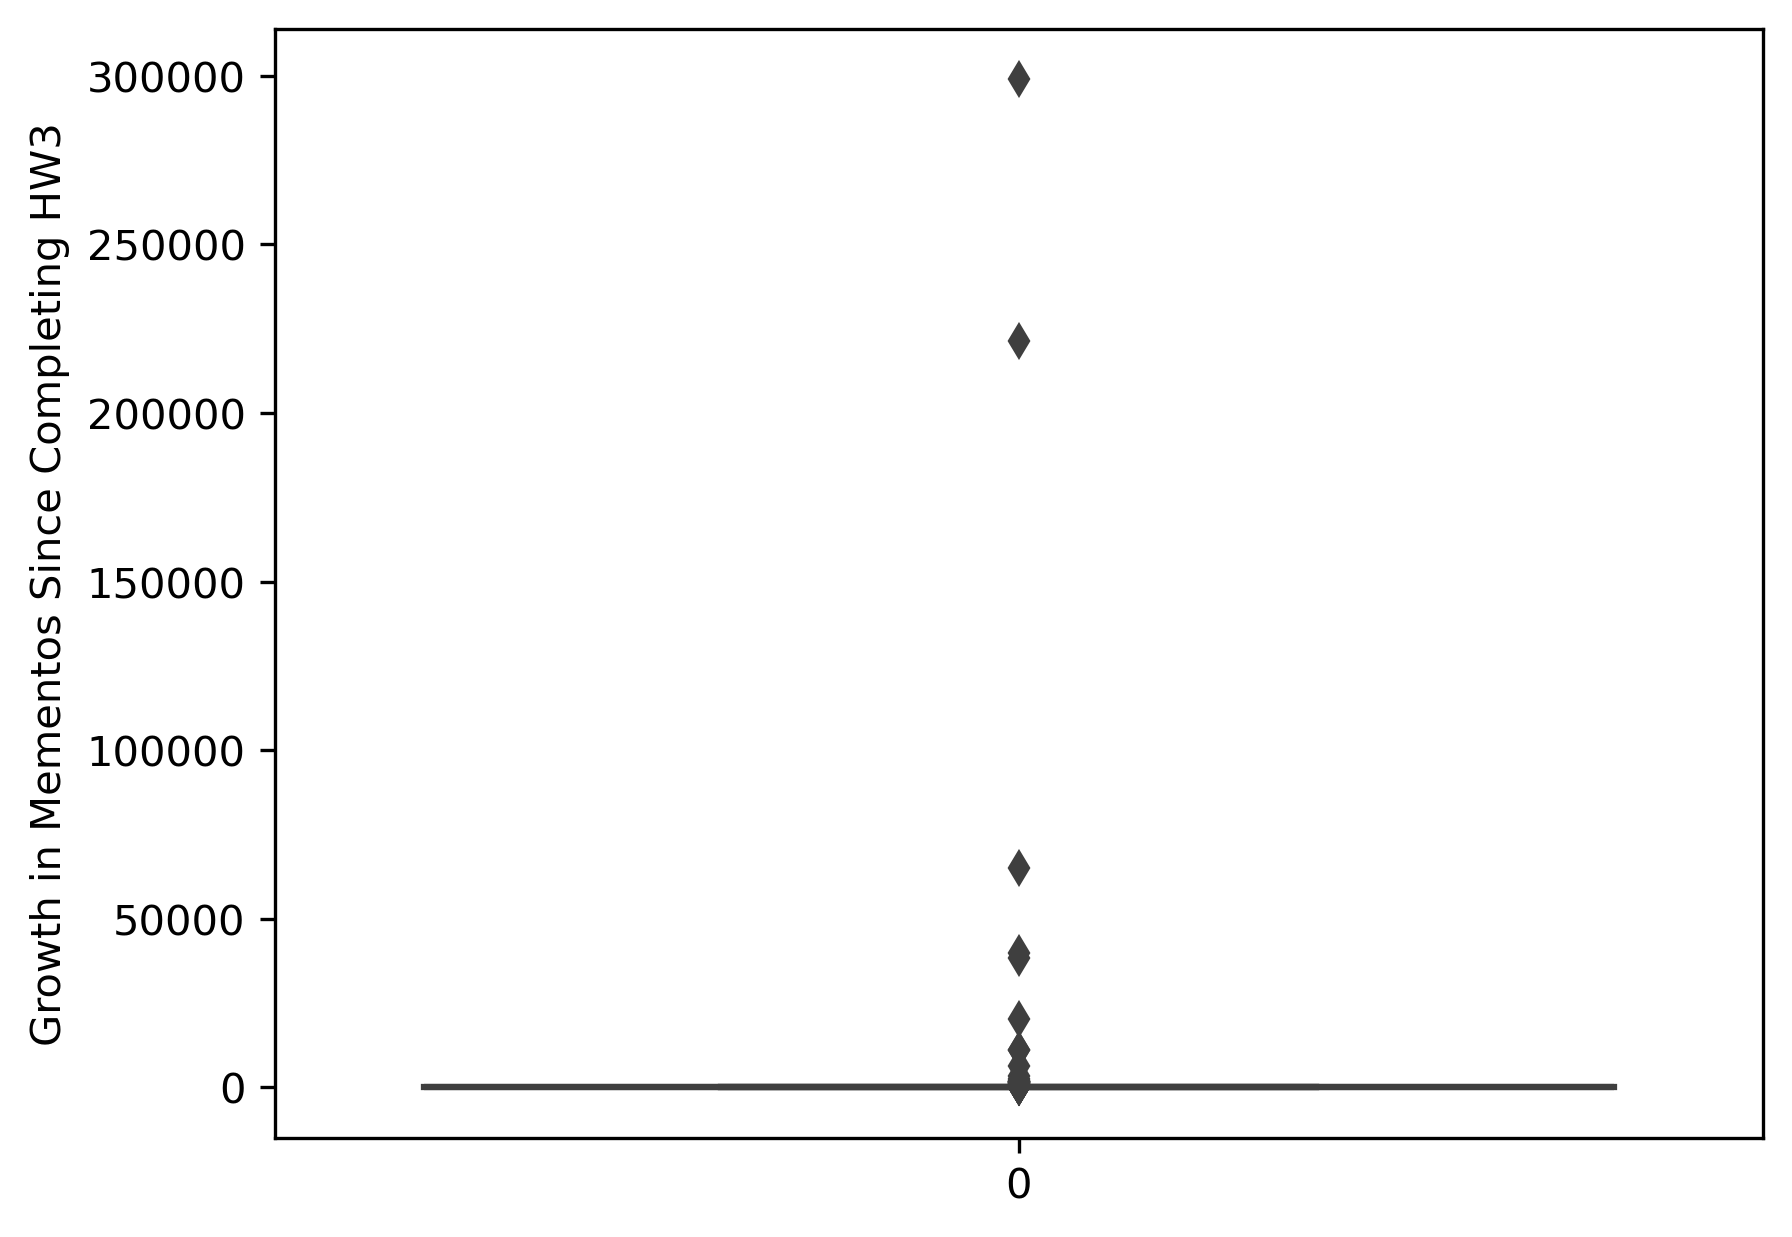
\includegraphics[width=\textwidth]{memento_growth_boxplot.png}
    \caption{Boxplot of the TimeMap Memento Count Differences}
    \label{fig:boxplot}
\end{figure}

%--------------------- Q2 ---------------------%

\clearpage

\section*{Q2}

To re-download the HTML for each webpage and remove the boilerplate, I started by duplicating the download-html.py and process-html.py from HW2. I then updated the paths in these scripts to ensure proper input and output directories were used. I ran each script to download the raw HTML and process it to remove the boilerplate. For consistency, I kept both sets of files (raw HTML and processed content) in separate folders as required and uploaded them to my class GitHub repository.

\emph{Q: Do all 500 URIs still return a "200 OK" as their final response (i.e., at the end of possible redirects)?}

To verify the status of the URIs, I created a script named check\_status\_codes.py to check the HTTP response codes of each URI. The script takes as input the URI mapping file generated by download-html.py, which contains all the relevant URIs to HW2 and this assignment. The script uses a dictionary to store the status codes for each URI and a Counter collection to tally different response categories (200OK or non-200 OK). Depending on the status code received, the appropriate counter is incremented.

After processing, the script saves the status codes to a file named status\_codes.json for use in later questions in HW9. Additionally, the script outputs a summary of the status codes to provide a quick overview of the results. Upon running the script, I found that 505 URIs returned 200 OK responses while 24 URIs returned non-200 OK responses.


%--------------------- Q3 ---------------------%

\section*{Q3}

I created a script named compare\_webpage\_sizes.py to compare the sizes of resulting text from HW2 and the current text. To achieve this, I first implemented a function called get\_file\_sizes.py to compute the sizes of all files in a given directory in bytes. I then supplied four directories to this function to retrieve the file sizes for both the raw and processed HTML files from HW2 and the current work. After calculating the differences in sizes for both raw and processed HTML sizes, I plotted the results as boxplots for visualization (refer to Figure \ref{fig:q3}).

\begin{figure}
    \centering
    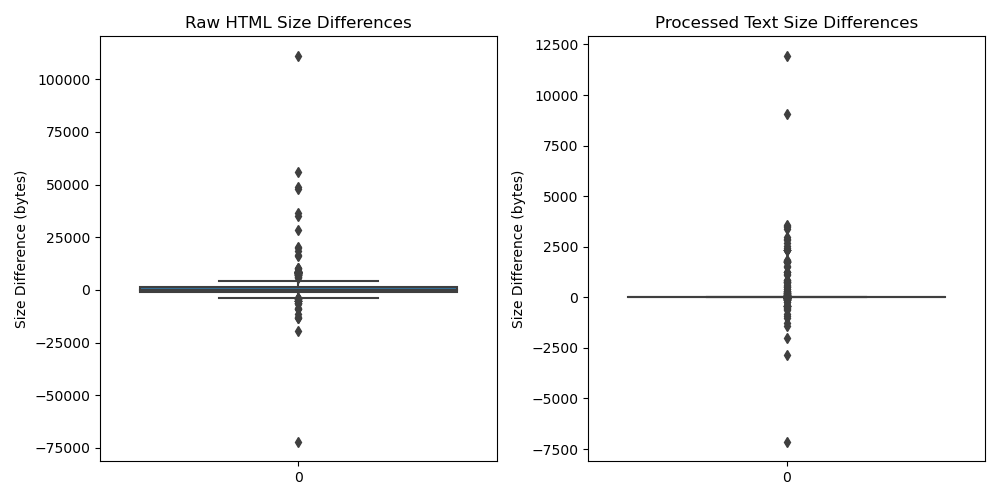
\includegraphics[width=1\linewidth]{q3.png}
    \caption{Raw and Processed HTML Text Size Differences}
    \label{fig:q3}
\end{figure}

Overall, there was a noticeable increase in text size between the completion of HW2 and the current work for both raw and processed HTMLs. While some shrinkage occurred in text size for both types, the growth was more significant. Notable outliers include one raw HTML that grew by 100,000 bytes and another that decreased by 75,000 bytes.

%--------------------- Q4 ---------------------%

\section*{Q4}

I created a script named explore\_webpage\_differences.py to analyze the top three URIs that exhibited the most significant changes. This script utilized the JSON file generated by check\_status\_codes.py as the source of the status codes for Q4. I began by filtering the URIs to include only those that returned a 200 OK response. 

Next, the script iterated through these filtered URIs to compare the sizes of the processed files from HW2 and the current assignment. The size differences were calculated, sorted in descending order, and the top three URIs with the largest changes were selected. Below are the output statistics generated by the script:

\begin{verbatim}
Top 3 URIs with the most significant changes:
27e75055b4c3c78a42f7b280bfa64e92.html: 11964 bytes
b10c01549227c83825e3c82761084462.html: 9046 bytes
1787bbdde8554a5efd2c2d27d75fec61.html: 7134 bytes
\end{verbatim}

In the same script, I used the difflib Python library to inspect line-by-line the differences between the top three URIs. The first URI corresponds to Old Dominion University, where the output shows outdated information was removed and replaced with new, relevant details about university operations. The second URI appears to belong to a music hall, where similar updates were made to reflect timely and relevant content. The final URI hosts abstracts of certain publications, and the differences suggest a new abstract was added to the page.

%----------------- References -----------------%

\clearpage

\section*{References}

\begin{itemize}
    \item {difflib.unified\_diff, \url{https://docs.python.org/3/library/difflib.html}}
    \item {Matplotlib 3.9.3 documentation, \url{https://matplotlib.org/stable/index.html}}
    \item {os.path, \url{https://docs.python.org/3/library/os.path.html}}
    \item {Python Counter Collection Documentation, \url{https://docs.python.org/3/library/collections.html#collections.Counter}}
    \item {Python Requests Library Documentation, \url{https://docs.python-requests.org/en/latest/user/quickstart/#response-status-codes}}
\end{itemize}

\end{document}